\documentclass[aspectratio=169]{beamer}
\usepackage[utf8]{inputenc}

% design
\usetheme{CambridgeUS}
\usecolortheme{beaver}
\setbeamertemplate{itemize items}[square]
%\setbeamercolor{itemize items}{fg=red}
\usenavigationsymbolstemplate{\beamertemplatenavigationsymbolsempty}

% bibliography
\usepackage{natbib}
\usepackage{har2nat}
\bibliographystyle{unsrt}

% tikz
\usepackage{tikz}
\usetikzlibrary{positioning}

% maths
\usepackage{amsmath}
\usepackage{amssymb}
\usepackage{amsthm}
\theoremstyle{definition}
\newtheorem{defn}{Definition}

% useful math symbols
\newcommand{\PR}{\mathbb{P}}
\newcommand{\E}{\mathbb{E}}
\newcommand{\V}{\operatorname{Var}}
\newcommand{\eqdist}{\overset{d}{=}}
\newcommand{\I}[1]{\mathbb{I}\{#1\}}
\newcommand{\Ntoinfty}{\overset{N\to\infty}{\longrightarrow}}
\newcommand{\limNtoinfty}{\underset{N\to\infty}{\lim}}
\newcommand\indep{\protect\mathpalette{\protect\independenT}{\perp}}
\def\independenT#1#2{\mathrel{\rlap{$#1#2$}\mkern2mu{#1#2}}}

% distributions
\newcommand{\N}{\mathcal{N}}
\newcommand{\Cat}{\operatorname{Categorical}}
\newcommand{\Unif}{\operatorname{Uniform}}
\newcommand{\Mn}{\operatorname{Multinomial}}
\newcommand{\Bin}{\operatorname{Binomial}}

% project-specific commands
\newcommand{\F}{\mathcal{F}_{t-1}}
\newcommand{\vt}[2][t]{v_{#1}^{(#2)}}
\newcommand{\wt}[2][t]{w_{#1}^{(#2)}}
\newcommand{\wbar}[2][t]{\bar{w}_{#1}^{(#2)}}
\newcommand{\vttilde}[2][t]{\tilde{v}_{#1}^{(#2)}}

\title[SMC Genealogies]{Asymptotic Genealogies of Sequential Monte Carlo Algorithms}
\author{Suzie Brown}
\date{26 April 2019} 

\begin{document}
\begin{frame}
\maketitle
\end{frame}

\begin{frame}{State space models}
\begin{columns}
\begin{column}{0.45\textwidth}
Hidden process $X_0, \dots, X_T \in \mathcal{X}$\\
Observable process $Y_0, \dots, Y_T \in \mathcal{Y}$\\[20pt]
\begin{center}
\begin{tikzpicture}
\node (yt) {$Y_t$};
\node (thet) [below=of yt] {$X_t$};
\node (yt1) [left=of yt] {$Y_{t-1}$};
\node (thet1) [below=of yt1] {$X_{t-1}$};
\node (dot1) [left=of thet1] {$\dots$};
\node (dot2) [right=of thet] {$\dots$};
\draw[->](thet.north)--(yt.south) node[midway, right] {\footnotesize{$g$}};
\draw[->](thet1.north)--(yt1.south) node[midway, right] {\footnotesize{$g$}};
\draw[->](thet1.east)--(thet.west) node[midway, above] {\footnotesize{$f$}};
\draw[->](dot1.east)--(thet1.west) node[midway, above] {\footnotesize{$f$}};
\draw[->](thet.east)--(dot2.west) node[midway, above] {\footnotesize{$f$}};
\end{tikzpicture}
\end{center}
\end{column}
\pause
\begin{column}{0.45\textwidth}
\begin{align*}
& X_0 \sim \mu(\cdot) \\
& X_{t+1} \mid (X_t = x_t) \sim f(\cdot | x_t)\\
& Y_t \mid (X_t = x_t) \sim g(\cdot | x_t)
\end{align*}
\end{column}
\end{columns}
\end{frame}

\begin{frame}{Target tracking}
\begin{columns}
\begin{column}{0.6\textwidth}
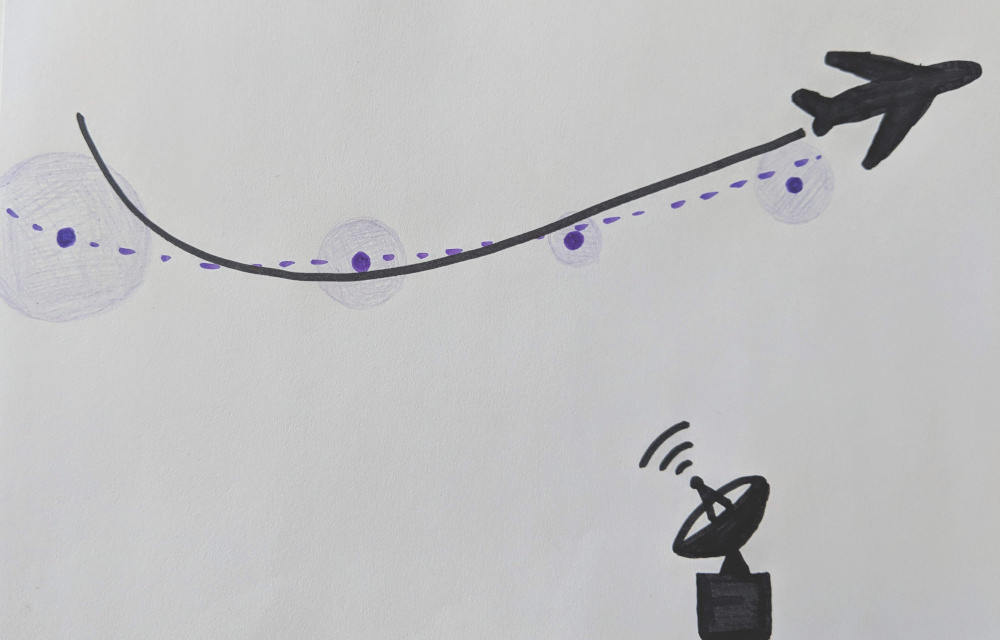
\includegraphics[width=\textwidth]{../tracking.jpg}
\end{column}
\begin{column}{0.35\textwidth}
use noisy radar data to infer position/trajectory of aircraft:
\begin{itemize}
\item $f$ models how aircraft moves
\item $g$ models uncertainty in radar measurements
\end{itemize}
\end{column}
\end{columns}
\end{frame}

\begin{frame}{Inference problems}
\textbf{Filtering:} where is it now? $p(x_{t} | y_{0:t})$\\[7pt]
\textbf{Prediction:} where will it go next? $p(x_{t+1} | y_{0:t})$\\[7pt]
\textbf{Smoothing:} where has it been? $p(x_{0:t} | y_{0:t})$\\[12pt]

Smoothing is ``harder'' than filtering/prediction \cite{gordon1993}. 
\end{frame}

\begin{frame}{Deterministic solutions}
\begin{columns}
\begin{column}{0.45\textwidth}
{\Large Kalman filter \cite{kalman1960}}\\
Under a linear Gaussian model:
\begin{align*}
& X_0 \sim \N(0, \Sigma_0) \\
& X_{t+1} \mid (X_t = x_t) \sim \N(A x_t, \Sigma_x) \\
& Y_t \mid (X_t = x_t) \sim \N(B x_t, \Sigma_y)
\end{align*}
we can recursively compute filtering distributions. 
Then a backward pass of RTS smoother \cite{rauch1965} provides smoothing distributions.\\[7pt]
This class of models is rather restrictive.
\end{column}
\pause
\begin{column}{0.45\textwidth}
{\Large Extended Kalman filter \cite{jazwinski2007}}\\
In non-linear Gaussian models, use a local linear approximation and apply Kalman filter.\\[7pt]
This requires gradients and performs poorly in models that are very non-linear.\\[12pt]
\pause
{\Large Unscented Kalman filter \cite{wan2000}}\\
For highly non-linear Gaussian models, replace the prediction step of Kalman filter by propagating a representative set of points through $f$.
\end{column}
\end{columns}
\end{frame}

\begin{frame}{Deterministic solutions}
\begin{itemize}
\item Kalman filter is optimal for linear Gaussian models, but extended/unscented Kalman filter are no longer optimal.\\[7pt] %%% what does optimal even mean?
\pause
\item All of these methods require a Gaussian model.
Deterministic solutions are available for some other conjugate families \cite{vidoni1999}, but these are still restrictive. \\[7pt]
\pause
\item Solutions are also available in the case that $\mathcal{X}$ is finite (integrals become sums), but we will mostly consider $\mathcal{X}$ to be a continuous space. \\[7pt]
\end{itemize}
\pause
Sequential Monte Carlo (SMC) provides general-purpose (stochastic) methods that do not require a tractable model.\\[7pt]
\pause 
Only requires sampling from $f(\cdot | x)$, and pointwise evaluation of $g(y | x)$ up to a normalising constant for each $y$.
\end{frame}

\begin{frame}{Sequential Monte Carlo}
\textbf{Prior: }
$p(x_{0:t}) = \mu(x_0) \prod_{i=1}^t f(x_i | x_{i-1})$ \\[7pt]
\textbf{Likelihood: }
$p(y_{0:t} | x_{0:t}) = \prod_{i=0}^t g(y_i | x_i)$ \\[7pt]
\textbf{Posterior: }
$p(x_{0:t} | y_{0:t}) \propto \mu(x_0) g(y_0 | x_0) \prod_{i=1}^t f(x_i | x_{i-1}) g(y_i | x_i)$\\[12pt]
\pause
\begin{itemize}
\item Represent posterior distribution at time $t$ with $N$ particles.\\[7pt]
\item Posterior factorises sequentially, avoiding increase of dimension with $T$.
\end{itemize}
\end{frame}

\begin{frame}{Sequential Monte Carlo}

{\Large Algorithm}\\
After initialisation, iterate these steps:
\begin{itemize}
\item \textbf{Propagate:} move the particles through the transition $f$
\item \textbf{Calculate weights:} weight each particle according to $g$
\item \textbf{Resample:} duplicate high-weight particles and kill off low-weight ones \\[12pt]
\end{itemize}
\pause
Approximate posterior distribution $p(dx_{0:t} | y_{0:t})$ by the empirical measure of the particles:
\begin{equation*}
\hat{p}(dx_{0:t}|y_{0:t}) = \frac{1}{N} \sum_{i=1}^N \delta_{X_{0:t}^{(i)}} (dx_{0:t})
\end{equation*}
\end{frame}

\begin{frame}{Ancestral degeneracy}
\begin{columns}
\begin{column}{0.35\textwidth}
For smoothing we need a sample of trajectories.\\[7pt]
Resampling means that trajectories of time $T$ particles coalesce backwards in time.
\end{column}
\begin{column}{0.6\textwidth}
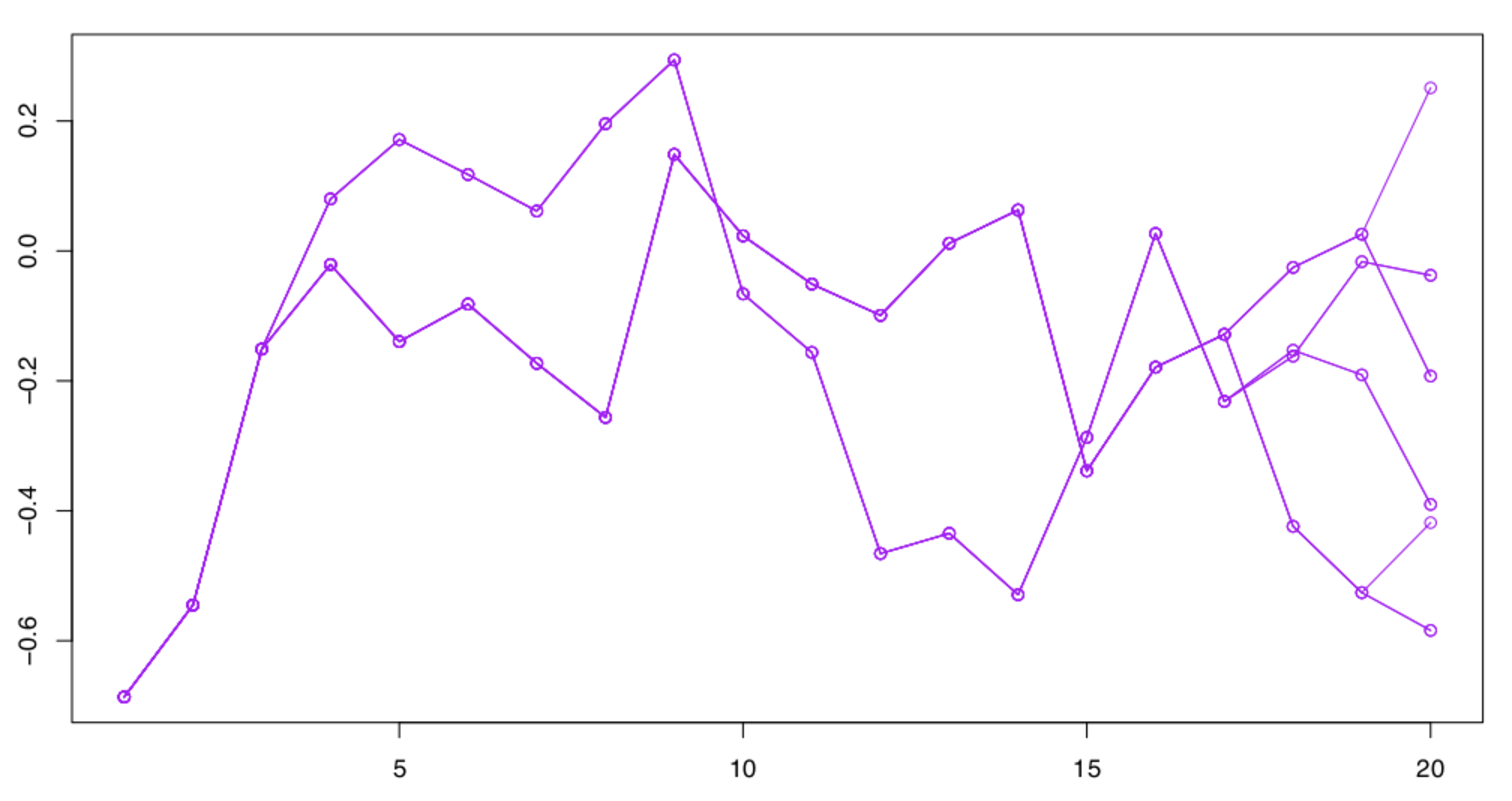
\includegraphics[width=\textwidth]{../degeneracy.pdf}
\end{column}
\end{columns}
\end{frame}

\begin{frame}{Kingman's coalescent}
\begin{columns}
\begin{column}{0.45\textwidth}
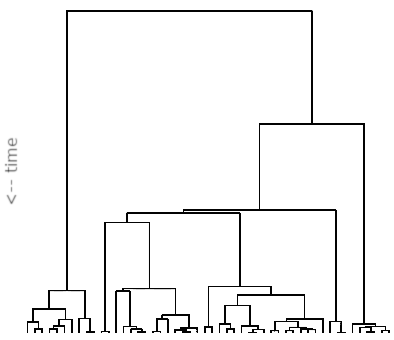
\includegraphics[width=\textwidth]{../kingman.png}
\end{column}
\begin{column}{0.45\textwidth}
Looking backwards in time, each pair of lineages coalesces with unit rate.\\[7pt]
\pause
This is the limiting coalescent process in many population models as $N\to\infty$ \cite{kingman1982coal, mohle1998}.
\end{column}
\end{columns}
\end{frame}

\begin{frame}{Coalescent for SMC}
\begin{itemize}
\item Analysing the coalescent can help us to understand the performance of various SMC algorithms.
\item The limiting coalescent of an SMC algorithm may depend on the resampling mechanism.
\item For multinomial resampling, the limiting coalescent is a scaled Kingman coalescent \cite{koskela2018}.
\item What about other (more used) resampling schemes?
\end{itemize}
\end{frame}

\begin{frame}{Resampling}
Requirements:\\[12pt]
\begin{itemize}
\item The total number of particles $N$ remains fixed. 
\item The particles after resampling are equally weighted. 
\item The resampling scheme is unbiased; that is, the expected number of offspring of each particle $i$ is equal to $N\wt{i}$.
\end{itemize}
\end{frame}

\begin{frame}{Resampling}
\textbf{Multinomial:}
$\vt{1:N} \eqdist \operatorname{Multinomial}(N, \wt{1:N})$\\[12pt]
\pause
\textbf{Residual \cite{liu1998}:}
$\vt{1:N} \eqdist \lfloor N \wt{1:N} \rfloor +  \operatorname{Multinomial}(R, r_t^{(1:N)}/R)$\\[7pt]
$\qquad r_t^{(i)} := (N \wt{i} - \lfloor N \wt{i}\rfloor)$\\[7pt]
$\qquad R:= \sum r_t^{(i)}$\\[12pt]
\pause
\begin{itemize}
\item Residual resampling yields lower Monte Carlo variance than multinomial resampling \cite{douc2005}.
\item Residual resampling is widely used by practitioners.
\item Analysing the coalescent for residual resampling is a work in progress.
\end{itemize}
\end{frame}

\begin{frame}{Particle Gibbs \citep{andrieu2010}}
Hidden Markov model where transition depends on a hyperparameter $\theta$:
\begin{align*}
& \theta \sim \nu(\cdot) \\
& X_0 \sim \mu(\cdot) \\
& X_{t+1} \mid (X_t = x_t) \sim f_{\theta}(\cdot | x_t)  \qquad t=0,\dots,T-1 \\
& Y_t \mid (X_t = x_t) \sim g(\cdot | x_t) \qquad t=0,\dots,T
\end{align*}
\pause
\textbf{Gibbs sampler:} alternately sample from $p(\theta | x_{0:t}, y_{0:t})$ and $p(x_{0:t} | \theta, y_{0:t})$.\\[7pt]
\pause
\begin{itemize}
\item SMC is an appropriate method for sampling from $p(x_{0:t} | \theta, y_{0:t})$
\item To target the correct posterior distribution, need to use \emph{conditional SMC}.
\end{itemize}
\end{frame}

\begin{frame}{Conditional SMC}
\begin{itemize}
\item One ``immortal'' trajectory is conditioned to survive all of the resampling steps.
\item Intuitively, this could have a significant effect on the coalescent. 
\pause
\item But we have this result:
\end{itemize}
\begin{block}{Corollary 1}
\textit{Under the conditions of \cite[Lemma 3]{koskela2018}
, the genealogy of any $n$ particles from a conditional SMC algorithm with multinomial resampling converges to Kingman's $n$-coalescent in the sense of finite-dimensional distributions, under an appropriate time-scaling.}
\end{block}
\pause
\begin{itemize}
\item Intuition: as $N\to\infty$, there is zero probability that an arbitrary sample of fixed size $n$ contains the immortal particle.
\end{itemize}
\end{frame}

\begin{frame}{Summary}
\begin{itemize}
\item SMC is widely used, but doesn't perform well for smoothing.
\pause
\item Analysis of SMC coalescents allows us to quantify the problem of ancestral degeneracy.
\pause
\item Proved: SMC with multinomial resampling $\Rightarrow$ Kingman coalescent.
\item (And simulations suggest it is a good model even for small $N$.)
\pause
\item Proved: conditional SMC (with multinomial resampling) $\Rightarrow$ Kingman coalescent.
\item In progress: investigate by simulations whether this is a good model for finite $N$.
\pause
\item In progress: analysis of residual resampling (and other resampling schemes).
\end{itemize}
\end{frame}

\begin{frame}[allowframebreaks]{References}

{\small 
\bibliography{../../smc.bib}
}
\end{frame}
\end{document}